

%Marketing materials are often generated to promote an entity (i.e., organization, person) and 
%persuade the audience about the information being conveyed. 
%instigate audience action. Because marketing campaigns are often multimodal, congruence in the promotional multimodal content is likely critical for effectiveness. 
To achieve contextual congruence, we utilize external knowledge from ConceptNet to incorporate in learning multimodal representations of data. We train knowledge embedding models described below to generate knowledge representations of concepts. First, we begin with defining contextual congruence, followed by description of our dataset.
% Below we identify several technical details that contribute to our analysis, including the definition of key terminology and the marketing data set we used.

% \subsection{Contextual Congruence.}
% \label{sec:context-congruence}

% Contextual congruence refers to the alignment and integration of information across multiple modalities (such as images, text, audio, etc.). It involves capturing the relationships and dependencies between different modalities to enhance the understanding and representation of the data. In that sense, contextual congruence aims to leverage each modality to create a unified representation that combines the strengths of each %modality 
% while preserving the inherent relationships between them.

\subsection{Contextual Congruence}
\label{sec:context-congruence}

Contextual congruence refers to the association between
%ability of human intelligence to form associations in the presence of 
multiple cues from different modalities, known to enhance human response accuracy
%behavior such as increasing accuracy in human responses 
\cite{laurienti2004semantic,spence2011crossmodal}. Recent research suggests that contextual congruence in crossmodal space facilitates the selection and processing of semantically related information from different modalities \cite{almadori2021crossmodal,laurienti2004semantic,letts2022evaluating}. 
%Hence, the richness of 
Multimodality 
%brings the challenge of 
challenges computational modeling, as the semantic cues
%contextual cues span across these modalities to make the meaning of the 
span across modalities to construct meaning. 
%While human brain learns to capture semantics between modalities, identifying these contextual connections is also critical in learning the representation of the holistic true meaning for machine. 
%As contextual congruency improves the human behavioral responses to the events, a similar mechanism for machine can be designed to achieve improvements. 
Given the goal of predicting human response to multimodal campaigns, capturing holistic meaning is essential. 

% \cite{hou2018semantic}


% \subsection{ConceptNet Knowledge Graph}
% \label{sec:concept-net-embedding-models}

% ConceptNet: ConceptNet is an open-source, multilingual knowledge graph that captures general world knowledge and semantic relationships between concepts. It connects words and phrases of natural language (terms) with labeled, weighted edges (relations). It aims 
% %most of all 
% to cover frequently-used words and phrases of every language and to represent generally-known relationships between the meanings of these terms.





% RotateE based on Euler’s identity, defines relations as a rotation from head to tail. It maps the head and tail entities $h, t$ to complex embeddings, i.e., $ h,t \approx C^{k}$. The functional mapping is induced by each relation r as an element-wise rotation from the head entity $h$ to the tail entity $t$. 
% The score function of RotateE measures the angular distance between head and tail elements and is defined as:
% https://math.stackexchange.com/questions/20412/element-wise-or-pointwise-operations-notation
% \begin{equation}
% d_r(h,t)=\lVert h\circ r - t \rVert
% \end{equation}


\begin{figure}[hbt!]
\vspace{-1.2em}
  \centering
  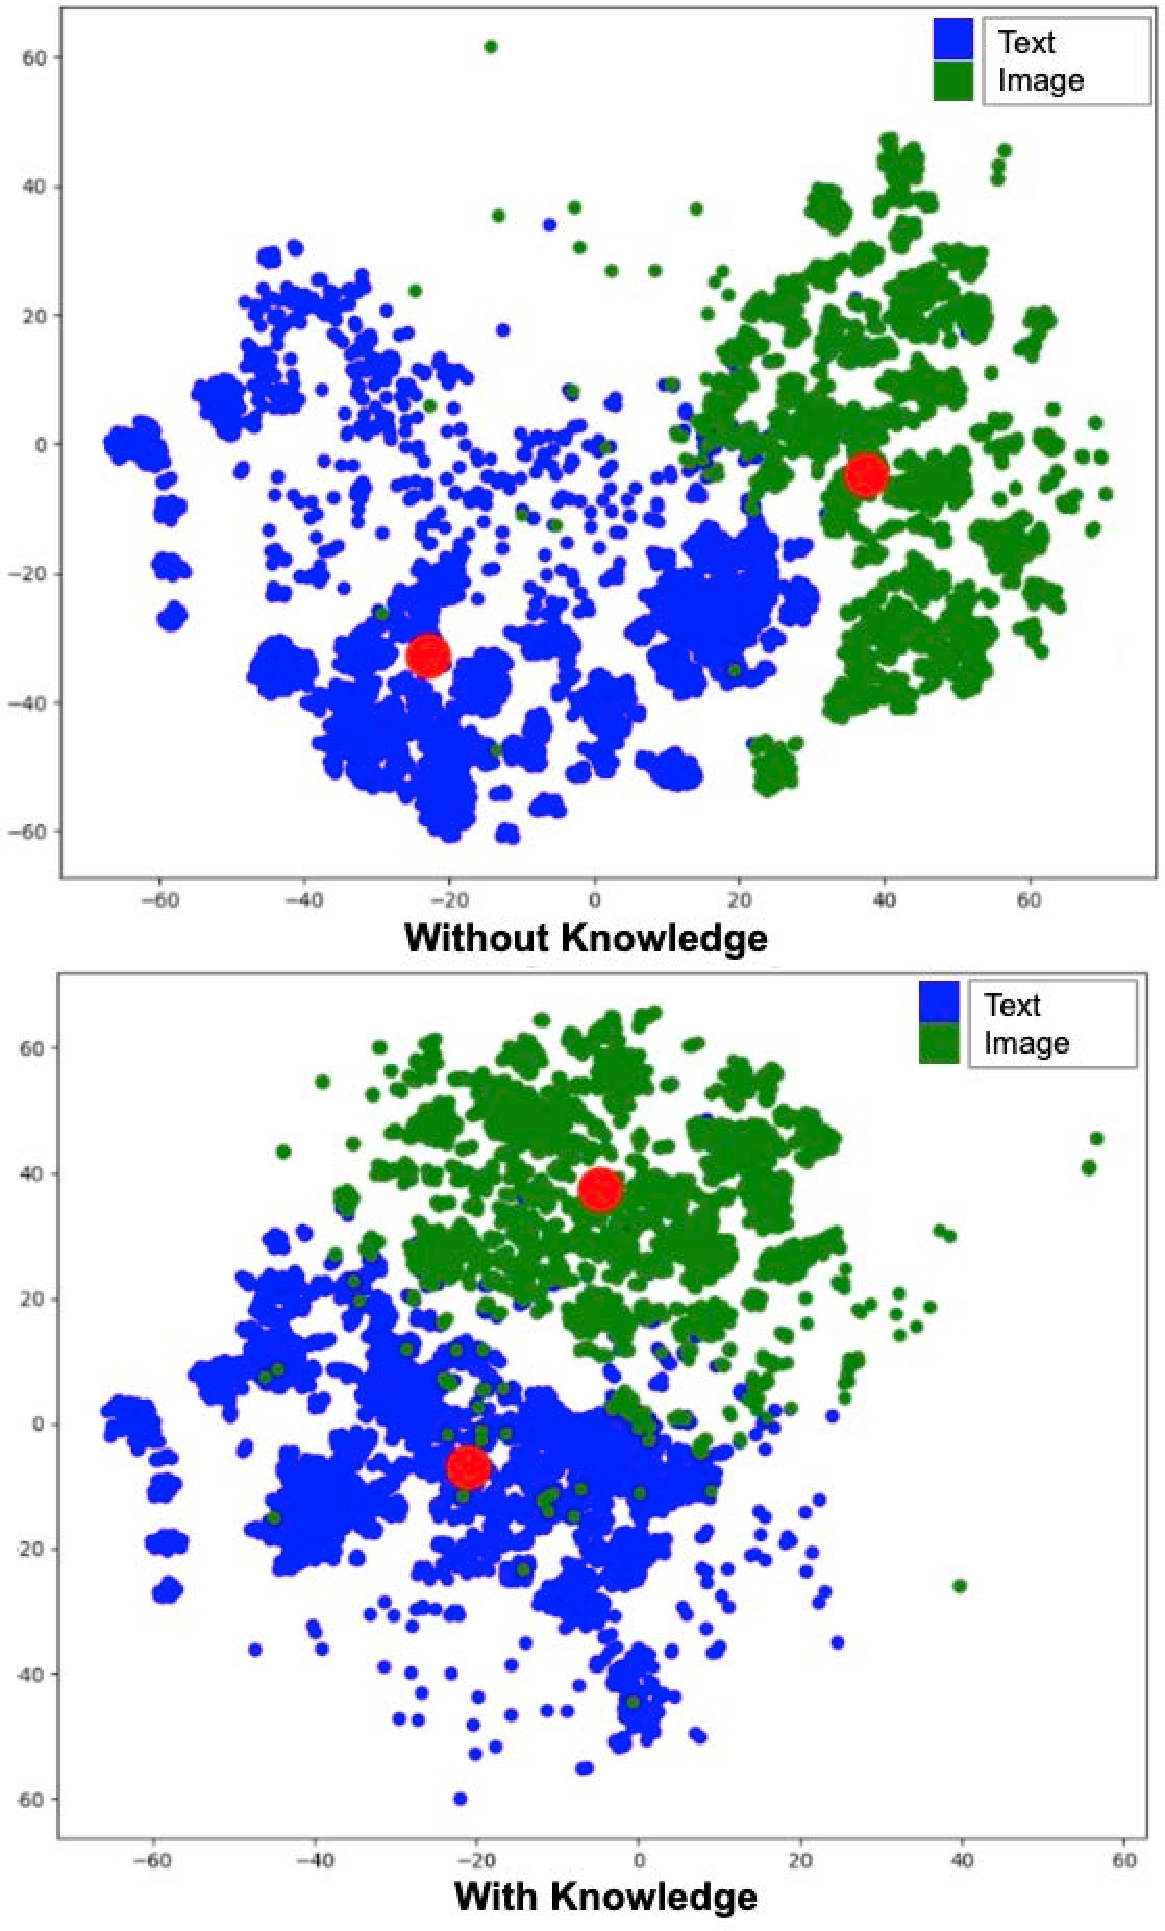
\includegraphics[width=8.3cm]{Figures/congruence_cluster_vertical.pdf}
\vspace{-1em}
\caption{t-SNE visualization of text and image caption (BLIP) embeddings as two clusters. The red dots represent the centroids in each cluster. The two clusters get denser and the distance between the text and image clusters reduces when we include concepts that we extracted from ConceptNet based on text and image captions.}
\vspace{-1.5em}
\label{fig:embds-cluster}
\end{figure} 


\subsection{Dataset}
\label{sec:dataset}

We have chosen the Kickstarter crowdfunding platform for its promotional multimodal content, where we have a valid outcome measure with a relatively large N. We utilize a dataset from Web Robots \cite{robots2018kickstarter} that collects data on  Kickstarter campaigns 
%with information regarding 
including attributes such as categories, goals, amount funded, the backers count, country, project type, and project URLs, among others. 

% The dataset will be made available and will fully comply with the FAIR principles \cite{force11}.

%through 
Kickstarter is an online crowdfunding platform where creators, entrepreneurs, designers, and artists, initiate promotional campaigns to seek resources for their creative projects in various categories. A campaigner introduces the concept behind their project in a project description. To back up their campaign, they frequently post videos, images, and text ads. Each project has a funding target with a deadline for a successful campaign. A project only receives the funds if it achieves or surpasses its funding target by the deadline going by the \textit{all-or-nothing} principle. 

We chose a one-year time frame between June 2021 and May 2022, and randomly sampled 75,810 Kickstarter projects. 
%We consider the promoted projects as successful if they were able to reach the funding target by the deadline, otherwise unsuccessful. 
%(when we performed our analysis) 
% restricting our dataset to only those projects which had reached their last date of fund collection. 
%The projects that make up the subject of study in this paper have all passed the deadline for receiving funding. 
% \textcolor{red}{Something wrong here---last sentences not in the PDF} 
A project is considered successful if it reaches its funding target by the deadline. Our binary outcome (dependent) variable represents whether the project was successful or unsuccessful.
In our dataset, 60.63\% were unsuccessful while 39.37\% were successful. 
% Thus we had a fairly balanced dataset for statistical analysis. %Response Variable (dependent measure) 




